\documentclass[a4paper,12pt,oneside]{book}
\usepackage[T1]{fontenc}                                      
\usepackage[utf8]{inputenc}                               
\usepackage[italian]{babel}
\usepackage{amsfonts}
\usepackage{amsthm}
\usepackage{amsmath,amssymb}
\usepackage{array}
\usepackage{arydshln}
\usepackage{braket}
\usepackage{blindtext}
\usepackage{calc}
\usepackage{cancel}
\usepackage{caption}
\usepackage{epsfig}
\usepackage{eucal}
\usepackage{fancyhdr}
\usepackage{geometry}
\usepackage{graphicx}
\usepackage{indentfirst}
\usepackage{hhline}
\usepackage{hyperref}
\hypersetup{
			colorlinks=true,
			linkcolor=black,
			anchorcolor=black,
			citecolor=black,
			urlcolor=black,
			pdftitle={Appunti di Meccanica Quantistica},
			pdfauthor={Vittorio Lubicz}
}

\usepackage{latexsym}
\usepackage{listings} 
\usepackage{longtable}
\usepackage{makeidx}
\usepackage{mathrsfs}
\usepackage{mathdots}
\usepackage{multirow}
\usepackage{nicefrac}
\usepackage{pdfpages}
\usepackage{physics}
\usepackage{setspace}
\usepackage{tikz}
\usepackage{tikz-3dplot}
\usepackage{textcomp}
\usepackage{titlesec,color}
\usepackage{vmargin}
\setpapersize{A4}
\setmarginsrb{35mm}{30mm}{35mm}{30mm}%
             {0mm}{10mm}{0mm}{10mm}



\definecolor{gray75}{gray}{0.75}
\newcommand{\hsp}{\hspace{20pt}}

\titleformat{\chapter}[hang]{\huge\bfseries}{\myfont{\textit{\large{\chaptername\hspace{1pt} \thechapter\hspace{3pt}}}}\textcolor{gray75}{$\mid$}\hspace{0.4cm}}{0pt}{\myfont{\huge\bfseries}}

\titleformat{\section}[hang]{\large\bfseries}{\myfont{\textit{\normalsize{\thesection\hspace{2pt}}}}\hspace{0.4cm}}{0pt}{\myfont{\Huge\bfseries}}

\titleformat{\subsection}[hang]{\large\bfseries}{\myfont{\textit{\small{\thesubsection\hspace{2pt}}}}\hspace{0.4cm}}{0pt}{\myfont{\huge\bfseries}}

\renewcommand{\chaptermark}[1]{\markboth{#1}{}}
\renewcommand{\sectionmark}[1]{\markright{#1}}
\newcommand*{\myfont}{\fontfamily{ppl}\selectfont}

\begin{document}

%*****************LAYOUT PAGINE**************************
\fancypagestyle{plain}{%
\fancyhf{} % cancella tutti i campi di  intestazione e pi\`e di pagina
\fancyfoot[C]{\bfseries \myfont{\thepage}} % tranne il centro
\renewcommand{\headrulewidth}{0pt}
\renewcommand{\footrulewidth}{0pt}}

\fancypagestyle{VS}{
\headheight = 15pt
\lhead[\myfont{\textit{\textbf{\thechapter\nouppercase{\leftmark}}}}]{\myfont{\textit{\textbf{\nouppercase{\leftmark}}}}}
\chead[]{}
\rhead[\myfont{\textbf{\thepage}}]{\myfont{\textbf{\thepage}}}

\lfoot[]{}
\cfoot[]{}
\rfoot[]{}
}
%*******************************************************



\pagestyle{VS}
\setcounter{chapter}{2}
\setcounter{page}{24}
\chapter[Formalismo Generale della M.Q.]{Formalismo Generale della Meccanica Quantistica: \\Ket, Bra e Operatori.\\Principio Di\\ Sovrapposizione.\\ Esperimenti di Stern e\\ Gerlach Ripetuti\footnote{F5.1-5.8,8.1-8.2; S1.1-1.3,1.5}}
 
Introduciamo qui \textbf{il formalismo generale} della meccanica quantistica descrivendo, in termini completamente quantistici, ancora un esperimento ideale. Questo esperimento è una generalizzazione di un famoso \textbf{esperimento}, realizzato da \textbf{Stern e Gerlach} nel 1921, che ha evidenziato la quantizzazione del momento angolare
 
\section{L'esperimento di Stern e Gerlach}
 L'esperimento di Stern-Gerlach aveva come obbiettivo la misura del momento magnetico degli atomi. Esso consiste nel far passare un fascio collimato di atomi di argento attraverso un campo magnetico non omogeneo. Un atomo di momento magnetico $\vec \mu$, che si trova in un campo magnetico di intensità $\vec B$, diretto lungo l'asse \emph{z}, acquista un'energia potenziale
\begin{equation}
V= -\vec \mu \cdot \vec B= -\mu_zB .
\end{equation} 

Se il campo magnetico non è omogeneo, ma la sua intensità varia lungo l'asse \emph{z}, allora l'atomo è soggetto ad una forza

\begin{equation}
F_z= - \frac{\partial V}{\partial z}= \mu_z\frac{\partial B}{\partial z} .
\end{equation}

Nell'esperimento di Stern e Gerlach il campo magnetico era orientato perpendicolarmente alla direzione di propagazione del fascio, dimodo che la forza \emph{F} devia gli atomi della loro traiettorie iniziali.

Secondo la \textbf{teoria classica}, tutte le orientazioni del momento magnetico sono ugualmente possibili e la forza \emph{F} può dunque assumere tutti i valori compresi tra $-\mu \frac{\partial B}{\partial z}$ e $+\mu \frac{\partial B}{\partial z}$. Atomi diversi verranno quindi differentemente deviati e si dovrebbe osservare, sullo schermo che intercetta il fascio, che questo si è uniformemente sparpagliato su una regione limitata tra un valore massimo e minimo di altezza.
\begin{center}
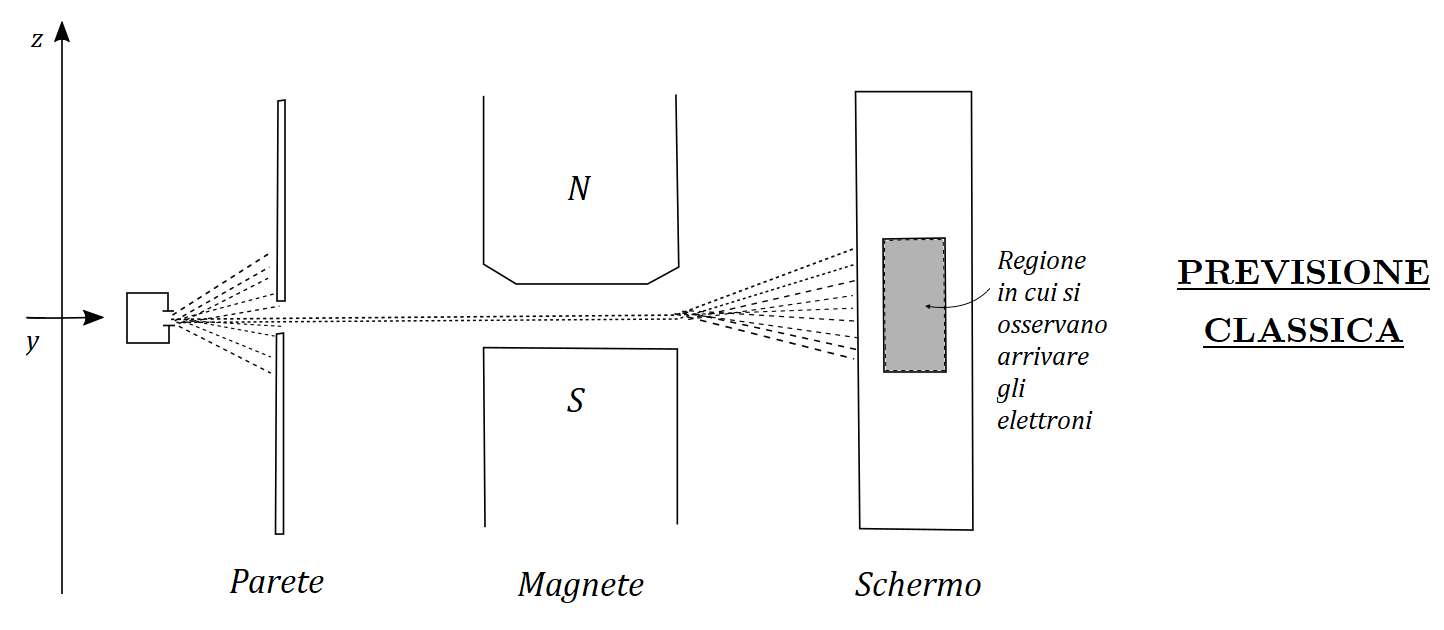
\includegraphics[width=11cm]{immagini/cap_3/fig_3_1.png}
\end{center}

Il \textbf{risultato dell'esperimento}, invece, fu completamente diverso dalle aspettative classiche: il fascio di atomi si separò perfettamente in due. Si osservò cioè che \textbf{il momento magnetico dell'atomo non può prendere che due orientazioni discrete:} $\mu_z=\pm \mu $ \\
\begin{center}
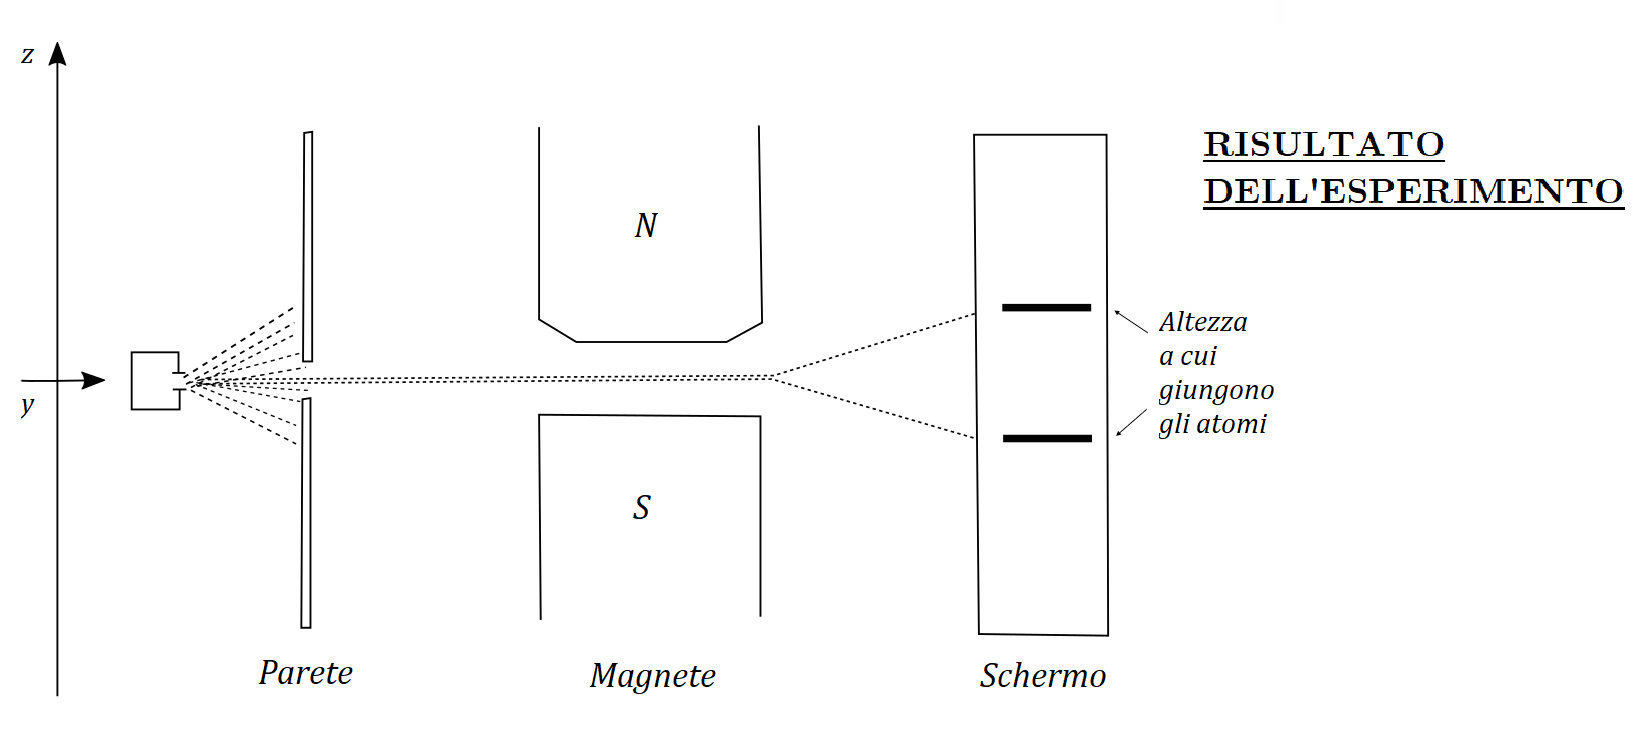
\includegraphics[width=11cm]{immagini/cap_3/fig_3_2.png}
\end{center}

L'atomo di argento è costituito da un nucleo e 47 elettroni, dei quali 46 possono essere visualizzati come una nube elettronica simmetrica priva di momento angolare complessivo. Se ignoriamo lo spin nucleare (che è accoppiato molto debolmente con il campo magnetico), vediamo che l'atomo nel suo complesso ha un momento angolare dovuto unicamente al momento angolare di spin (ossia "intrinseco") del solo 47-esimo elettrone. Poiché il momento magnetico risulta proporzionale al momento angolare, \textbf{il risultato dell'esperimento di Stern e Gerlach dimostra che il momento angolare di spin dell'elettrone è quantizzato, e la sua componente \emph{z} può assumere soltanto due valori discreti}. Questi valori sono:
\begin{equation}
S_z= \pm \frac{\hbar}{2}.
\end{equation}
 
\section{Esperimenti di Stern e Gerlach Ripetuti} 
Per discutere il formalismo generale della meccanica quantistica consideriamo una \textbf{versione modificata e ideale dell'esperimento di Stern e Gerlach.}
 
Consideriamo in primo luogo particelle di \textbf{Spin 1} che nell'attraversare un apparecchio di Stern e Gerlach, si separano in tre fasci: un fascio è deviato verso l'alto, uno verso il basso ed uno non viene affatto deflesso. La componente \emph{z} dello spin della particella può assumere i valori

\begin{equation}
S_z=0, \qquad S_z= \pm \hbar .
\end{equation}

consideriamo poi una versione modificata dell'apparecchio di Stern e Gerlach, rappresentata in figura \\
\begin{center}
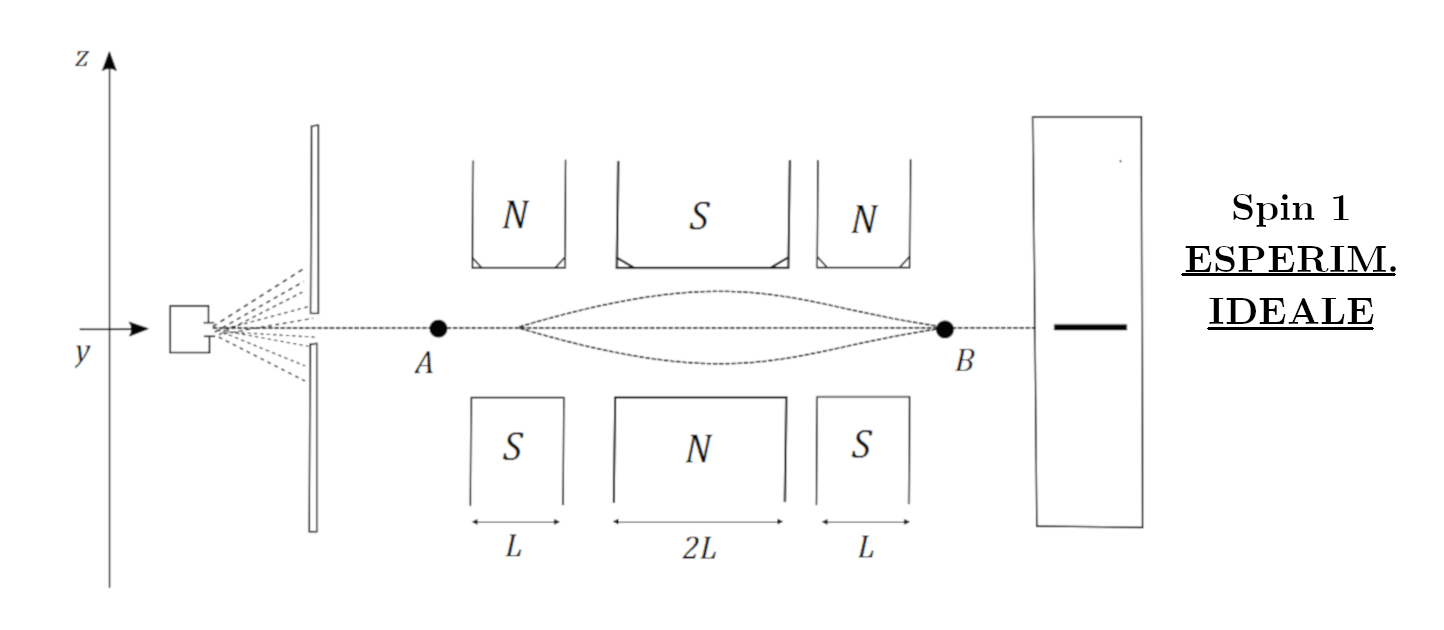
\includegraphics[width=11cm]{immagini/cap_3/fig_3_3.png}
\end{center}

Per la simmetria dell'apparecchio, il fascio di particelle che all'interno viene suddiviso in tre, esce comunque riunito.

Per concentrarci solo su fenomeni che dipendono dallo spin degli atomi, e non  dover includere effetti del moto sugli atomi, che escono fuori, supponiamo che all'ingresso dell'apparecchio in A ci sia un meccanismo che fa partire gli atomi da fermi, e all'uscita dell'apparecchio in B ci sia un altro meccanismo atto a fermare gli atomi e a riportarli a riposo in B.

Per brevità  di notazione, conveniamo di indicare l'apparecchi di Stern e Gerlach modificato con il simbolo.

\begin{equation}
\begin{Bmatrix} + \\ 0 \\ -  \end{Bmatrix}
\end{equation}
\begin{equation*}
S
\end{equation*}
 
 dove +, 0, - indicano i tre diversi fasci in cui si suddivide, all'interno, il fascio originario. Poiché ci proponiamo di usare molti apparecchi insieme, e con diverse orientazioni, li distingueremo ognuno con una lettera in basso ( \emph{S} nell'esempio precedente). Con degli opportuni diaframmi è possibile bloccare all'interno dell'apparecchio uno o più dei tre fasci, permettendo solo agli altri il proseguimento del percorso. Indicheremo per esempio l'apparecchio \\
\begin{center}
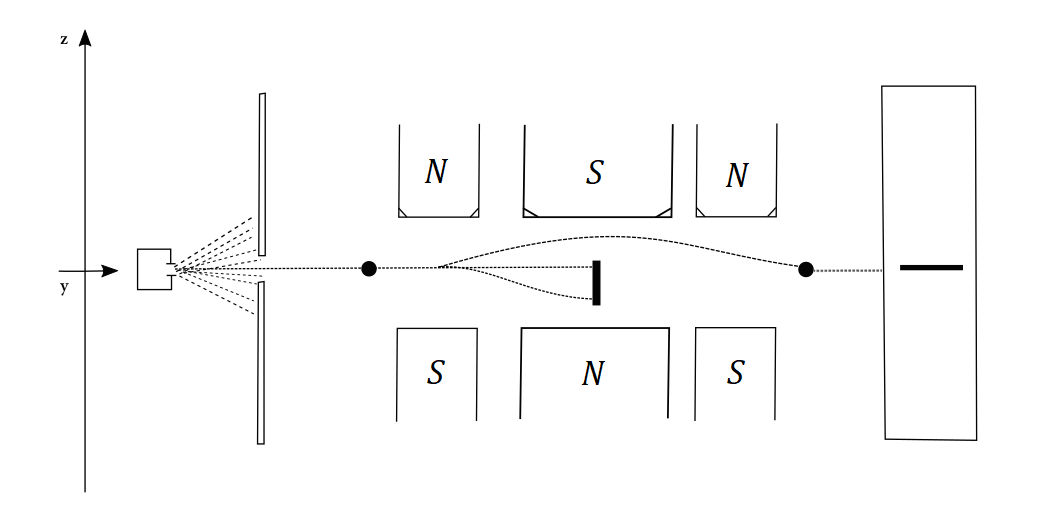
\includegraphics[width=10cm]{immagini/cap_3/fig_3_4.png}
\end{center}
 
con il simbolo
 
\begin{equation}
\begin{Bmatrix} + \\ 0\ | \\ -  |  
\end{Bmatrix}
\label{SG1}
\end{equation}
\begin{equation*}
S
\end{equation*}
 

 
Diremo che gli atomi che nell'apparecchio S passano nel fascio superiore sono \textbf{"nello stato più rispetto ad S"}, quelli che prendono il cammino di mezzo sono \textbf{"nello stato zero rispetto ad S"} e quelli che passano sotto \textbf{"nello stato meno rispetto ad S"}.

Un apparecchio di Stern e Gerlach con diaframmi, quale quello indicato in \eqref{SG1}, \textbf{è in grado di selezionare uno stato puro rispetto ad S}. Infatti con due apparecchi di Stern e Gerlach consecutivi, nella combinazione

\begin{equation}
\begin{Bmatrix}
 + \\ 0 | \\ - |  
\end{Bmatrix}
\begin{Bmatrix}
 + \\ 0 | \\ - |  
\end{Bmatrix} \qquad \text{SÌ}
\label{SG2}
\end{equation}
 
osserviamo che tutte le particelle che hanno attraversato il primo apparecchio attraversano pure il secondo. D'altro canto, con le due combinazioni di apparecchi

\begin{equation}
\begin{Bmatrix}
 + \\ 0 | \\ - |  
\end{Bmatrix}
\begin{Bmatrix}
 + |  \\ 0  \\ - |  
\end{Bmatrix} \qquad \text{NO}
\label{SG3}
\end{equation}

\begin{equation}
\begin{Bmatrix}
 + \\ 0 | \\ - |  
\end{Bmatrix}
\begin{Bmatrix}
 + |  \\ 0|  \\ -  
\end{Bmatrix} \qquad \text{NO}
\label{SG4}
\end{equation}

non si osserva nessuna particella in (non si capisce).

Abbiamo già discusso come, secondo la meccanica quantistica, la probabilità di un evento in un esperimento ideale è data dal modulo quadro di un numero complesso detto \textbf{ampiezza di probabilità}.

Per le ampiezze di probabilità utilizziamo la \textbf{la notazione inventata da Dirac} ed applicata usualmente in meccanica quantistica, secondo cui si indica con 
\begin{equation}
\langle\beta |\alpha \rangle ,
\end{equation} 

\textbf{l'ampiezza che un atomo, inizialmente nello stato $\alpha$, finisca nello stato $\beta$}, o, come anche si dice, che un atomo dallo stato $\alpha$ si porti nello stato $\beta$.

Le espressioni da (\ref{SG2}) a (\ref{SG4}) indicano per le ampiezze le relazioni

\begin{equation}
\langle +S |+S \rangle =1, \quad \langle 0S | +S \rangle =0, \quad \langle -S | +S \rangle=0 .
 \label{cap3_1}
\end{equation} 

Supponiamo di utilizzare due apparecchi di Stern e Gerlach in serie dei quali il secondo sia ruotato di un angolo $\alpha$ intorno all'asse \emph{y}. eseguiamo quindi i seguenti esperimenti ($T$ indica l'apparecchio ruotato)


\begin{eqnarray}
& &\begin{Bmatrix}
 + \\ 0 | \\ - |  
\end{Bmatrix}
\begin{Bmatrix}
 + \\ 0 | \\ - |  
\end{Bmatrix} \qquad \text{SÌ}  \\
& & \quad S  \ \qquad T
\label{SG5} \nonumber
\end{eqnarray}
\begin{equation}
\langle +T | +S \rangle \neq 0 ;
\end{equation} 


\begin{eqnarray}
& &\begin{Bmatrix}
 + \\ 0 | \\ - |  
\end{Bmatrix}
\begin{Bmatrix}
 + | \\ 0 \\ - |  
\end{Bmatrix} \qquad \text{SÌ} \\
& & \quad S  \ \qquad T \nonumber
\label{SG6}
\end{eqnarray}
\begin{equation}
\langle 0T | +S \rangle \neq 0 ;
\end{equation} 

\begin{eqnarray}
& & \begin{Bmatrix}
 + \\ 0 | \\ - |  
\end{Bmatrix}
\begin{Bmatrix}
 + | \\ 0 | \\ -   
\end{Bmatrix} \qquad \text{SÌ} \\
& & \quad S  \ \qquad T \nonumber 
\label{SG7}
\end{eqnarray}
\begin{equation}
\langle -T | +S \rangle \neq 0 .
\end{equation}

Ne segue che \textbf{gli atomi che sono in uno stato definito rispetto ad S non sono in uno stato definito rispetto a \emph{T}.}
Si osserva inoltre che il filtrare uno stato puro di T fa perdere l'informazione circa lo stato precedente della particella. Questo è stato dimostrato dal seguente esperimento:
\begin{eqnarray}
& &\begin{Bmatrix}
 + \\ 0 | \\ - |  
\end{Bmatrix}
\begin{Bmatrix}
 + | \\ 0  \\ - |  
\end{Bmatrix}
\begin{Bmatrix}
 + | \\ 0  \\ - |  
\end{Bmatrix} \qquad \text{SÌ} \\
& & \quad S  \ \qquad T\ \qquad S \nonumber
\label{SG8}
\end{eqnarray}

o in termini di ampiezze:
\begin{equation}
\langle 0S | 0T \rangle \langle 0T | +S \rangle \neq 0 .
\end{equation}

In altri termini, gli atomi che escono da $T$ sono nello stato ($OT$) e non hanno memoria del fatto che prima erano nello stato ($+S$).

Questi risultati illustrano uno dei principi fondamentali della meccanica quantistica: \textbf{ogni sistema atomico può essere analizzato, per mezzo di un processo di filtraggio, in un certo insieme di stati, chiamati stati di base. Il comportamento futuro degli atomi che si trovao in un determinato stato di base dipende solo dalla natura di questo stato ed è indipendente dalla storia precedente.}

Gli stati di base dipendono, come è chiaro dal filtro che si è usato. Per esempio i tre stati ($+S$),($0S$) e($-S$) sono un insieme di stati di base, i tre stati ($+T$),($0T$) e($-T$) un altro. Si parla comunemente di state di base in un certa \textbf{"rappresentazione"}.

Osserviamo che la perdita di informazione nell'esperimento (\ref{SG8}) è causata non dall'aver separato in tre il fascio nell'apparecchio $T$, ma dall'aver introdotto in $T$ dei diaframmi. Infatti si ha:

\begin{eqnarray}
& &\begin{Bmatrix}
 + \\ 0 | \\ - |  
\end{Bmatrix}
\begin{Bmatrix}
 +  \\ 0  \\ -   
\end{Bmatrix}
\begin{Bmatrix}
 + | \\ 0  \\ - |  
\end{Bmatrix} \qquad \text{NO} \\
& & \quad S  \ \qquad T\ \qquad S \nonumber
\label{SG9}
\end{eqnarray}

In generale un apparecchio $T$, o un altro qualsiasi non diaframmato non produce alcun cambiamento. Abbiamo già discusso come, in meccanica quantistica quando un evento può avvenire secondo varie altre motivazioni, l'ampiezza di probabilità per l'evento è la somma dell'ampiezza di probabilità per le varie alternative considerate separatamente. L'ampiezza di probabilità per l'esperimento (\ref{SG9}) si scrive allora

\begin{equation}
\sum\limits_{i=+,0,-}=\langle 0S | iT \rangle \langle iT | +S \rangle ,
\end{equation}

e questa ampiezza deve essere uguale a quella ottenuta rimuovendo  dall'esperimento l'apparecchio $T$ diaframmato. Dunque:
\begin{equation}
\sum\limits_{i=+,0,-}=\langle 0S | iT \rangle \langle iT | +S \rangle = \langle OS | +S \rangle .
 \label{cap3_2}
\end{equation}

La perdita di informazione sullo stato iniziale della particella nell'esperimento (\ref{SG8}) è dunque dovuto all'introduzione nell'apparecchio $T$ dei diaframmi di arresto, ossia all'aver eseguito una misura dello stato $T$ della particella. Questo risultato è generale ( e ne abbiamo visto un altro esempio nella discussione dell'esperimento di interferenza degli elettroni nel passaggio di due fenditure): \textbf{il processo di misura nella meccanica quantistica influisce sempre sulla particella, oggetto della misura. Questa proprietà è dovuta al fatto che le caratteristiche delle particella non si manifestano che come risultato della misura stessa}.
E' questa proprietà essenziale del processo di misura che giustifica il paradosso cui si giunge confrontando i risultati (\ref{SG8}) e (\ref{SG9}): \textbf{lasciando aperti più canali passano meno atomi} (si ha pertanto un esempio di interferenza distruttiva). Dal punto di vista matematico questo è conseguenza del fatto che in meccanica quantistica si sommano le ampiezze e non le probabilità.
Nel caso delle esperimento (\ref{SG8}) abbiamo

\begin{equation}
P= | \langle 0S | 0T \rangle \langle 0T | +S \rangle  |^2 \neq 0 .
\end{equation}

Nel caso (\ref{SG9}) invece

\begin{equation}
P= |\sum \limits_{i=+,0,-}\langle 0S | iT \rangle \langle iT | +S \rangle |^2 =0 ,
\end{equation}
(la somma delle ampiezze è nulla ma ciascuna delle tre ampiezze è diversa da zero).

Dimostriamo infine un'altra importante legge cui soddisfano le ampiezze. Abbiamo già visto come un apparecchio senza diaframmi non abbia alcuna influenza sullo stato della particella. Abbiamo allora che:
\begin{equation}
\sum \limits_{i=+,0,-}\langle +S | iT \rangle \langle iT | +S \rangle = \langle +S | +S \rangle =1 .
\end{equation}

D'altra parte la probabilità che una particella nello stato $| +S \rangle$ attraversando un apparecchio $T$ vada a passare attraverso uno qualsiasi dei tre fasci di $T$ deve essere 1, cioè

\begin{equation}
\sum \limits_{i=+,0,-}|\langle iT | +S \rangle|^2= \sum \limits_{i=+,0,-} \langle iT | +S \rangle ^* \langle iT | +S \rangle= 1 .
\end{equation}
dal confronto delle ultime due equazioni ricaviamo che, per ogni $i$

\begin{equation}
 \langle iT | +S \rangle ^* = \langle +S | iT \rangle .
 \label{cap3_3}
\end{equation}

Riepiloghiamo, esprimendole in forma generale \textbf{tre leggi importanti} ricavate per le ampiezze.
Queste sono contenute nelle equazioni (\ref{cap3_1}), (\ref{cap3_2}), (\ref{cap3_3})
\begin{enumerate}
\item $\langle i | j \rangle=\delta_ij$
\item $\langle \chi | \varphi \rangle=\sum \limits_{i} \langle \chi | i \rangle \langle i | \varphi \rangle$
\item $\langle \chi | \varphi \rangle \langle \varphi | \chi \rangle ^*$
\end{enumerate}

In queste equazioni $i$ e $j$ si riferiscono a \textbf{tutti} gli stati di base in una singola rappresentazione, mentre $\varphi$ e $\chi$ rappresentano due stati arbitrari della particella.

\section[Principio di sovrapposizione]{Vettori di stato BRA e KET. Principio di sovrapposizione} 

Le equazioni sin qui derivate per le ampiezze di probabilità quantistiche presentano una forte rassomiglianza formale cone le proprietà del prodotto scalare di due vettori.

Per esempio l'equazione

\begin{equation}
\langle \chi | \varphi \rangle =\sum \limits_{i}\langle \chi | i \rangle \langle i | \varphi \rangle
\label{cap3_4}
\end{equation}

può essere paragonata con la formula valida per il prodotto scalare di due vettori $\vec{B}$ ed $\vec{A}$:

\begin{equation}
\vec{B} \cdot \vec{A}= \sum \limits_{i} (\vec{B} \cdot  \vec{e_i})(\vec{e_i} \cdot \vec{A}) ,
\label{cap3_5}
\end{equation}

dove $\vec{e_i}$ sono i tre versori di base nelle dimensioni $x,y,z$. Infatti $\vec{B}\cdot \vec{e_1=B_x}$, $\vec{B}\cdot \vec{e_2=B_y}$,$\vec{B}\cdot \vec{e_3=B_z}$ (e analoghe per  $\vec{A}$) e (\eqref{cap3_5}) è equivalente a:

\begin{equation}
\vec{B} \cdot \vec{A} = B_xA_x+B_yA_y+B_zA_z .
\end{equation}

Confrontando le equazioni (\ref{cap3_4}) e (\ref{cap3_5}) si vede che gli stati $\varphi$ e $\chi$ corrispondono ai due vettori $\vec{A}$ e $\vec{B}$ e gli stati di base $i$ corrispondono ai vettori di base $\vec{e_i}$.

Poiché i vettori di base $\vec{e_i}$ sono ortonormali, vale la relazione

\begin{equation}
\vec{e_i} \cdot \vec{e_j}= \delta_{ij} .
\end{equation}

Questa relazione ha il suo analogo nell'equazione

\begin{equation}
\langle i | j \rangle = \delta_{ij} ,
\end{equation}

valida per le ampiezze di transizione tra stati di base.

C'è una differenza tra le ampiezze quantistiche ed il prodotto scalare. Per le prime si ha che

\begin{equation}
\langle \varphi | \chi \rangle = \langle \chi | \varphi\rangle ^* ,
\label{cap3_6}
\end{equation} 

mentre, nell'algebra dei vettori, 

\begin{equation}
\vec{A} \cdot \vec{B}= \vec{B} \cdot \vec{A} ,
\label{cap3_7}
\end{equation}

ossia, nel prodotto scalare l'ordinamento dei termini è irrilevante.

L'equazione (\ref{cap3_5}), che esprime una proprietà del prodotto scalare di due vettori, è valida in generale per qualunque vettore $\vec{B}$. L'equazione può quindi essere scritta in forma vettoriale "eliminando" $\vec{B}$ da entrambi i membri. Si arriva così all'equazione 

\begin{equation}
\vec{A} = \sum \limits_{i} \vec{e_i} (\vec{e_i}\cdot\vec{A}) \equiv \sum \limits_{i} A_i\vec{e_i}= A_x\vec{e_x}+A_y\vec{e_y}+A_z\vec{e_z} .
\end{equation}

In modo analogo si può pensare di definire dalla relazione quantistica (\ref{cap3_4}) l'analisi di un "vettore". Eliminando il $\langle \chi |$ da entrambi i membri della (\ref{cap3_4}) si ottiene

\begin{equation}
 | \varphi \rangle= \sum \limits_{i} | i \rangle \langle i | \varphi \rangle \equiv \sum \limits_{i} c_i | i \rangle .
\label{cap3_8}
\end{equation}

In altri termini: \textbf{la parentesi $\langle \chi | \varphi \rangle $ viene considerata composta di due parti. La seconda parte, $| \varphi \rangle $, è detta \emph{ket} mentre la prima, $\langle \chi |$, è detta \emph{bra}. La notazione è di Dirac. Insieme $\langle \chi |$ e $| \varphi \rangle$ compongono una \emph{bra-ket} ("bracket", parentesi in inglese). I simboli $\langle \chi |$ e $| \varphi \rangle$ sono anche detti vettori di stato}.

La differenza fra le equazioni (\ref{cap3_6}) e (\ref{cap3_7}) sta ad indicare che i vettori di stato ket ed i vettori bra sono definiti in uno \textbf{spazio vettoriale complesso}. In particolare, scriviamo l'equazione (\ref{cap3_8}) per un vettore $| \chi\rangle$:

\begin{equation}
| \chi \rangle = \sum \limits_{i} | i \rangle \langle i | \chi \rangle \equiv \sum \limits_{i} d_i | i \rangle .
\end{equation}

Confrontiamo questa equazione con quella che si ottiene dalla (\ref{cap3_4}) eliminando il ket $| \varphi \rangle$ ed utilizzando la proprietà (\ref{cap3_6}):

\begin{equation}
\langle \chi | =\sum \limits_{i} \langle \chi | i \rangle \langle i | = \sum \limits_{i} d^*_i \langle i | .
\end{equation}

Vediamo dunque che vale la seguente regola di corrispondenza tra ket e bra:

\begin{equation}
c_{\alpha}| \alpha \rangle +c_{\beta} | \beta \rangle  \leftrightarrow c^*_{\alpha}\langle \alpha | +c^*_{\beta}\langle \beta | .
\end{equation}

Sottolineiamo che mentre i vettori nello spazio a tre dimensioni sono rappresentabili per mezzo di tre versori mutuamente ortogonali, \textbf{i vettori di base $| i \rangle $per gli stati quantistici devono variare su quell'insieme completo che si adatta al particolare problema}. A seconda dei casi, possono essere necessarie due, o tre o anche un numero infinito di stati di base.

Consideriamo l'interpretazione fisica dell'equzione (\ref{cap3_8}). Essa afferma che, \textbf{in meccanica quantistica, ogni stato $| \varphi \rangle$ può essere espresso come combinazione lineare, o sovrapposizione, con opportuni coefficienti, di un insieme di stati di base. Viceversa, se lo stato $| \varphi \rangle$ e lo stato $| \chi \rangle$ sono due stati accessibili per il sistema, allora qualunque combinazione lineare di $| \varphi \rangle$ e $| \chi \rangle$ è ancora uno stato accessibile del sistema}. Questo enunciato costituisce il cosidetto \textbf{principio di sovrapposizione degli stati} e rappresenta uno dei principali fondamentali della meccanica quantistica.

\textbf{La possibilità per un sistema di trovarsi in uno stato che è una sovrapposizione di più stati è un concetto puramente quantistico e non ha analogo classico}. Così un atomo può trovarsi in una sovrapposizione di stati di spin, un fotone in una sovrapposizione di stati di polarizzazione, un elettrone in uno stato risultante dalla sovrapposizione di stati che definiscono il passaggio attraverso una o l'altra di due fenditure. E' il principio di sovrapposizione che è dunque alla base di tutti i fenomeni di interferenza sin qui considerati.

Concludiamo con un'osservazione sulla \textbf{normalizzazione} dei vettori di stato. Scegliamo nell'equazione (\ref{cap3_4}) lo stato arbitrario $| \chi \rangle$ uguale allo stato $| \varphi \rangle$ troviamo che:

\begin{equation}
\langle \varphi | \varphi \rangle = \sum \limits_{i} \langle \varphi | i \rangle \langle i | \varphi \rangle = \sum \limits_{i} |\langle i | \varphi \rangle |^2 ,
\end{equation}

ossia l'ampiezza $\langle \varphi| \varphi \rangle$ è sempre un numero reale, ma negativo. Il quadrato di questa ampiezza rappresenta la probabilità che "un sistema nello stato $| \varphi \rangle$ venga trovato nello stato $\langle \varphi | \varphi \rangle $. Tale probabilità è evidentemente uguale a 1. L'ampiezza $\langle \varphi| \varphi \rangle$ deve dunque soddisfare

\begin{equation}
\langle \varphi| \varphi \rangle =1 .
\end{equation}

I vettori di stato corrispondenti a stati fisici devono essere \textbf{normalizzati}.

\section[Operatori]{Operatori. Rappresentazioni Matriciali e relazione di completezza}

Per introdurre il concetto di "operatore" consideriamo nuovamente un esperimento di Stern e Gerlach ideale costituito nel modo seguente:

\begin{eqnarray}
& &\begin{Bmatrix}
 + \\ 0 | \\ - |  
\end{Bmatrix}
\begin{Bmatrix}
\quad \\  A  \\ \quad
\end{Bmatrix}
\begin{Bmatrix}
 +| \\ 0  \\ - |  
\end{Bmatrix}\\
& & \quad S  \ \qquad \quad\ \qquad R \nonumber
\end{eqnarray}

Con $A$ si intende un qualunque insieme, comunque complicato, di apparecchi di Stern e Gerlach. La corrispondente ampiezza di probabilità che la particella, inizialmente nello stato $| +S \rangle$ prima di entrare in $A$, ne esca nello stato $| 0R \rangle$ si indica con

\begin{equation}
\langle 0R|A| +S \rangle .
\end{equation}

in generale $A$ indica \textbf{una qualunque operazione effettuata sullo stato della particella}, e si dice che $A$ \textbf{è un operatore}. Quando un operatore agisce su un vettore di stato la trasforma in un altro vettore di stato.

Per comprendere come l'apparecchio $A$ agisce tra una coppia di stati arbitrari consideriamo il seguente esperimento

\begin{eqnarray}
& &\begin{Bmatrix}
 + \\ 0 | \\ - |  
\end{Bmatrix}
\begin{Bmatrix}
  + \\ 0  \\ -   
\end{Bmatrix}
\begin{Bmatrix}
\quad \\  A  \\ \quad 
\end{Bmatrix}
\begin{Bmatrix}
  + \\ 0  \\ -   
\end{Bmatrix}
\begin{Bmatrix}
  +| \\ 0  \\ -|   
\end{Bmatrix} \\
& & \quad S  \ \qquad R\ \qquad  \ \qquad T\ \qquad R \nonumber
\end{eqnarray}
in cui ai lati dell'apparecchio $A$ sono aggiunti due apparecchi $T$ senza filtri. Poiché la presenza di apparecchi senza filtri non modifica la situazione dal punto di vista fisico, per le corrispondenti ampiezze abbiamo

\begin{equation}
\langle 0R|A| +S \rangle = \sum \limits_{i} \sum \limits_{j} \langle 0R | iT \rangle \langle iT | A | jT \rangle \langle jT | +S \rangle .
\end{equation}

Questa espressione non dipende evidentemente dalla specifica scelta dell'apparecchio $T$ e dalla scelta degli stati iniziale e finale, $| +S \rangle $ e $\langle OR |$. Può quindi essere scritta nella forma generale

\begin{equation}
\langle \chi | A | \varphi \rangle = \sum \limits_{i,j} \langle \chi | i \rangle \langle i | A | j \rangle \langle j | \varphi \rangle .
\label{cap3_9}
\end{equation}

Il secondo membro dell'equazione (\ref{cap3_9}) è in realtà più semplice del primo. Ci dice che \textbf{l'apparecchio $A$ è completamente descritto da nove numeri}

\begin{equation}
\langle i | A | j \rangle  \qquad \forall i,j ,
\end{equation}

che danno la risposta di $A$ relativa ai tre stati di base in una determinata rappresentazione. Una volta noti questi nove numeri è possibile calcolare l'azione dell'operatore $A$ tra due stati iniziali e finali $| \varphi \rangle $ e $| \chi \rangle$ qualsiasi se definiamo ciascuno di essi per mezzo delle tre ampiezze per la transizione a ($\langle j | \varphi \rangle $) o da ($\langle \chi | i \rangle$) ognuno dei tre stati di base.

L'equazione (\ref{cap3_9}) può essere anche scritta in forma vettoriale eliminando lo stato arbitrario $\langle \chi | $:

\begin{equation}
A| \varphi \rangle = \sum \limits_{i,j}  |i \rangle \langle i | A | j \rangle \langle j | \varphi \rangle .
\label{cap3_10}
\end{equation}

Questa equazione definisce completamente lo \textbf{sviluppo in termini dei vettori di base $ | i \rangle$ del vettore di stato $A | \varphi \rangle $} ottenuto facendo agire l'operatore $A$ sul ket $ | \varphi \rangle$.

Analogamente, eliminando lo stato $\varphi$ nell'equazione (\ref{cap3_9}) possiamo derivare l'effetto di un operatore $A$ che agisce su un bra $ \langle \chi |$ da destra:

\begin{equation}
\langle \chi | A\ = \sum \limits_{i,j} \langle \chi | i \rangle \langle i | A  | j \rangle \langle j | .
\label{cap3_11}
\end{equation}

Questa equazione definisce \textbf{lo sviluppo del bra $\langle \chi |A$ in termini dei ket di base $\langle j |$}.

Tutti gli operatori che consideriamo qui sono operatori lineari.

Risulta spesso conveniente raccogliere i diversi numeri complessi $\langle i | A | j \rangle$ che definiscono l'azione dell'operatore $A$ nella forma di una \textbf{matrice quadrata} $N\times N$, dove $N$ è in generale la dimensione dello spazio de ket ($N=3$ per gli atomi di spin 1 nell'esperimento di Stern e Gerlach):

\begin{equation}
A \doteq
\begin{pmatrix}
\langle 1 | A  | 1 \rangle & \langle 1 | A  | 2 \rangle & \cdots\\
\langle 2 | A  | 1 \rangle & \langle 2 | A  | 2 \rangle & \cdots \\
\cdots & \cdots & \cdots \\
\end{pmatrix} .
\end{equation}

Il simbolo $\doteq$ sta per "è rappresentato da"

Osserviamo che gli elementi di questa matrice dipendono evidentemente dalla particolare scelta effettuata per i vettori di base $| i \rangle$.

I coefficienti dello sviluppo del vettore di stato

\begin{equation}
| \psi \rangle \equiv A | \varphi \rangle ,
\end{equation}

in termini dei ket di base possono essere ottenuti moltiplicando entrambi i membri dell'equazione (\ref{cap3_10}) a sinistra per un bra di base $\langle k | $:

\begin{equation}
\langle k | \psi \rangle = \langle k | A | \varphi \rangle \equiv \sum \limits_{i,j} \langle k | i \rangle \langle i | A | j\rangle \langle j | \varphi \rangle = \sum \limits_{j} \langle k | A | j \rangle \langle j | \varphi \rangle ,
\end{equation}

dove si è utilizzata l'ortonormalità dei vettori di base: $\langle k | i \rangle =\delta_{ki}$. Ma questa equazione può essere vista come l'ordinario \textbf{prodotto di una matrice per un vettore colonna} quando i coefficienti dello sviluppo dei vettori di stati $| \varphi \rangle$ e $| \psi \rangle =A | \varphi \rangle$ sono disposti nella forma di vettore colonna.

\begin{equation}
| \varphi \rangle \doteq 
\begin{pmatrix}
\langle 1 | \varphi \rangle \\
\langle 2 | \varphi \rangle \\
\vdots \\
\end{pmatrix}, \qquad
| \psi \rangle \doteq 
\begin{pmatrix}
\langle 1 | \psi \rangle \\
\langle 2 | \psi \rangle \\
\vdots \\
\end{pmatrix} .
\end{equation}

Analogamente, i coefficienti dello sviluppo del bra

\begin{equation}
\langle \gamma | = \langle \chi | A ,
\end{equation}
ottenuto facendo agire (da destra) l'operatore $A$ sul bra $\langle \chi | $, possono essere ottenuti moltiplicando scalarmente l'equazione (\ref{cap3_11}) per il ket di base $| k \rangle$:

\begin{equation}
\langle \gamma | k \rangle = \langle \chi | A | k \rangle \equiv \sum \limits_{i,j}  \langle \chi | i \rangle \langle i | A | j \rangle  \langle j | k \rangle = \sum \limits_{i} \langle \chi | i \rangle  \langle i | A | k \rangle .
\end{equation}

Questa equazione può essere ora interpretata come l'ordinario \textbf{prodotto di un vettore riga per una matrice} quando conveniamo di rappresentare i bra $ \langle \gamma |$ e  $\langle \chi |$ in termini di vettori riga:

\begin{equation}
\langle \chi | \doteq 
\begin{pmatrix}
\langle \chi | 1 \rangle && \langle \chi | 2 \rangle && \cdots 
\end{pmatrix}
 = 
\begin{pmatrix}
\langle 1 | \chi \rangle ^* && \langle 1 | \chi \rangle ^* && \cdots
\end{pmatrix} ,
\end{equation}

\begin{equation}
\langle \gamma | \doteq 
\begin{pmatrix}
\langle \gamma | 1 \rangle && \langle \gamma | 2 \rangle && \cdots 
\end{pmatrix}
 = 
\begin{pmatrix}
\langle 1 | \gamma \rangle ^* && \langle 2 | \gamma \rangle ^* && \cdots
\end{pmatrix} .
\end{equation}

Si noti in queste espressioni la comparsa dell'operazione di coniugazione complessa.

Con una notazione matriciale può essere anche espresso il prodotto scalare di due vettori di stato $\langle \chi |$ e $ | \varphi \rangle $. Scriviamo questo prodotto nella forma:

\begin{equation}
\langle \chi | \varphi \rangle = \sum \limits_{i} \langle \chi | i \rangle \langle i | \varphi \rangle .
\end{equation}

Questo non è altro che \textbf{il prodotto di un vettore riga per un vettore colonna}:

\begin{equation}
\langle \chi | \varphi \rangle = 
\begin{pmatrix}
\langle 1 | \chi \rangle ^* & \langle 2 | \chi \rangle ^* & \cdots 
\end{pmatrix} 
\begin{pmatrix}
\langle 1 | \varphi \rangle \\ 
\langle 2 | \varphi \rangle 
\\ \vdots 
\end{pmatrix} .
\end{equation}

Un operatore particolarmente semplice è \textbf{l'operatore identità $I$}, definito come l'operatore la cui azione su un qualunque vettore di stato è nulla:

\begin{equation}
\langle \chi | I | \varphi \rangle \equiv \langle \chi | \varphi \rangle .
\end{equation}

Confrontando questa relazione con l'equazione (\ref{cap3_4}), se ne deduce che è possibile scrivere per gli stati di base

\begin{equation}
\sum \limits_{i} \langle i | i \rangle = I .
\end{equation}

Questa equazione è nota come \textbf{relazione di completezza}.

La relazione di completezza, unità all'equazione

\begin{equation}
\langle i | j \rangle =\delta_{ij} ,
\end{equation}

garantisce che gli stati $\langle i | $ costituiscano un buon sistema di base.

Calcoliamo questo paragrafo osservando che in generale è possibile definire il prodotto di un ket per un bra nella forma

\begin{equation}
| \alpha \rangle \langle \beta |  ,
\end{equation}

e viene detto \textbf{prodotto esterno} (come contrapposto al prodotto scalare di un bra per un ket detto anche prodotto interno).

Il prodotto esterno è evidentemente un operatore, ed i suoi elementi di matrice in una determinata rappresentazione si ottengono moltiplicando (come in ogni altro caso) l'operatore per il bra di base $\langle i |$ a sinistra ed il ket di base $| j \rangle$ a destra:

\begin{equation}
| \alpha \rangle \langle \beta | \doteq
\begin{pmatrix}
\langle 1 | \alpha \rangle \langle 1 | \beta \rangle ^* && \langle 1 | \alpha \rangle \langle 2 | \beta \rangle ^* && \cdots \\
\langle 2 | \alpha \rangle \langle 1 | \beta \rangle ^* && \langle 2 | \alpha \rangle \langle 2 | \beta \rangle ^* &&  \cdots \\
\vdots && \vdots && \ddots
\end{pmatrix} .
\end{equation}

\section{Prodotto di Operatori}

Riferendoci nuovamente ad un esperimento di Stern e Gerlach consideriamo un apparecchio, che chiameremo $C$, costituito da due apparecchi $A$ e $B$ posti in serie:

\begin{equation}
\begin{Bmatrix}
C
\end{Bmatrix}=
\begin{Bmatrix}
A
\end{Bmatrix}
\begin{Bmatrix}
B
\end{Bmatrix} .
\end{equation}

L'azione dell'apparecchio $C$ può essere studiata inserendo un apparecchio senza filtri tra $A$ e $B$. Per due stati iniziali e finali arbitrari, $| \varphi \rangle $ e $\langle \chi |$, si ha allora

\begin{equation}
\langle \chi | C | \varphi \rangle = \sum \limits_{i} \langle \chi | B | i \rangle \langle i | A | \varphi \rangle .
\label{cap3_12}
\end{equation}

Questa equazione può essere espressa nella forma di un'identità operatoriale utilizzando la relazione di completezza e l'arbitrarietà degli stati esterni:

\begin{equation}
C= B \cdot A .
\end{equation}

\textbf{L'operatore risultante dall'applicazione successiva di due operatori, $A$ e $B$, è dunque il prodotto degli operatori $B \cdot A$.}

Sostituendo nell'equazione (\ref{cap3_12}) gli stati esterni $\langle \chi |$ e $ | \varphi \rangle $ con due vettori di base $\langle j |$ e $| k \rangle$ si ottengono mediante l'usuale \textbf{prodotto riga per colonna} degli elementi di matrice corrispondenti agli operatori $B$ ed $A$ rispettivamente:

\begin{equation}
\langle j | C | k \rangle  = \sum \limits_{i} \langle j | B | i \rangle \langle i | A | k \rangle .
\end{equation}

Ne segue immediatamente che il prodotto di due operatori non gode della proprietà commutativa ossia in generale

\begin{equation}
A \cdot B \neq B \cdot A . 
\end{equation}

\section{Cambiamenti di Base e Trasformazioni Unitarie}

Abbiamo già osservato come la scelta di un determinato insieme di vettori di base non è univoca ed in generale, anzi, \textbf{esistono infinite possibili scelte di vettori di base o, come si dice anche, di rappresentazioni.}

E' evidente come \textbf{due scelte differenti }implicano la comparsa, nei calcoli di \textbf{diverse componenti di vettore} per la rappresentazione degli stati, e di \textbf{diversi elementi di matrice} per la rappresentazione di operatori (ad esempio $\langle i | \varphi \rangle $ o  $ \langle i | A | j \rangle $).

\textbf{Tuttavia}, se il formalismo sin qui sviluppato è consistente la risposta finale circa il risultato \textbf{di una misura qualsiasi deve essere sempre la stessa.}

Discutiamo qui in dettaglio come si effettua un \textbf{cambiamento di base} e quindi sono le relazioni tra elementi di vettori e di matrici in due basi differenti.

Consideriamo due diverse possibili scelte di vettori di base che indicheremo, per poterli distinguere chiaramente, con 

\begin{equation}
| a^{(1)} \rangle , \quad  | a^{(2)} \rangle , \cdots , | a^{(N)} \rangle ,
\end{equation}
e
\begin{equation}
| b^{(1)} \rangle , \quad | b^{(2)} \rangle , \cdots , | b^{(N)} \rangle ,
\end{equation}
rispettivamente.

Ci poniamo in primo luogo di trovare un operatore $U$ che trasforma i vettori di base $| a^{(i)} \rangle$ nei vettori di base $| b^{(i)} \rangle $ , ossia 

\begin{equation}
| b^{(i)} \rangle \equiv U | a^{(1)} \rangle \qquad \forall i .
\end{equation}

La forma esplicita di questo operatore si ottiene prendendo il prodotto esterno di entrambi i membri di questa equazione con il $\langle a^{(1)}| $ e sommando su tutti gli $i$. Utilizzando la relazione di completezza troviamo allora:

\begin{equation}
\sum \limits_{i} | b^{(i)} \rangle \langle a^{(i)} |  = \sum \limits_{i} U | a^{(i)} \rangle \langle a^{(i)} |  = U ,
\end{equation}
 ossia
 
\begin{equation}
U = \sum \limits_{i} | b^{(i)} \rangle \langle a^{(i)} | .
\end{equation}

Calcoliamo esplicitamente la matrice rappresentativa dell'operatore $U$ nella base $\left\{ | a^{(i)} \rangle    \right\} $:

\begin{equation}
\langle a^{(i)} | U | a^{(j)} \rangle \equiv \sum \limits_{k} \langle a^{(i)} | b^{(k)} \rangle  \langle a^{(k)} | a^{(j)} \rangle  ,
\end{equation}

ossia, per la proprietà di ortonormalità $\langle a^{(k)} | a^{(j)} \rangle  =\delta_{k,j}$

\begin{equation}
\langle a^{(i)} | U | a^{(j)} \rangle \equiv \langle a^{(i)} | b^{(j)} \rangle .
\end{equation}

La matrice quadrata costruita da $\langle a^{(i)} | U | a^{(j)} \rangle $ è detta \textbf{matrice di trasformazione} dalla base $\left\{ | a^{(j)} \rangle  \right\}$ alla base $\left\{ | b^{(i)} \rangle  \right\}$. Le colonne di questa matrice sono costituite dai vettori rappresentativi degli stati di base $\left\{ | b^{(i)} \rangle  \right\}$ nella rappresentazione $\left\{ | a^{(i)} \rangle  \right\}$.

In generale, dato un operatore arbitrario $A$, si definisce \textbf{operatore hermitiano coniugato} di A, e lo si indica con il simbolo $A^+$, l'operatore tale che, per qualunque coppia di vettori $| \varphi \rangle$ e $ | \chi \rangle $ soddisfa

\begin{equation}
\langle \varphi | A^{+} | \chi \rangle = \langle \chi | A | \varphi \rangle ^* .
\label{cap3_13}
\end{equation}

Questa relazione implica, per gli elementi di matrice rappresentativa dell'operatore in una determinata base,

\begin{equation}
\langle i | A^{+} | j \rangle = \langle j | A | i \rangle ^* .
\end{equation}

Pertanto, la matrice che rappresenta l'hermitiano congiunto di un operatore $A$ si ottiene a partire dalla matrice che rappresenta $A$ considerandone la trasposta ed effettuando un'operazione di coniugazione complessa sugli elementi di matrice


Calcoliamo esplicitamente l'operatore hermitiano coniugato dell'operatore $U$. Dalla definizione di hermitiano coniugato si ha:

\begin{equation}
\langle \varphi | U^{+} | \chi \rangle = \langle \chi | U | \varphi \rangle ^* =  \left( \sum \limits_{i} \langle \chi | b^{(i)} \rangle \langle a^{(i)} | \varphi \rangle \right)^* =\sum \limits_{i} \langle \varphi | a^{(i)}\rangle \langle b^{(i)} | \chi \rangle ,
\end{equation}

da cui, per l'arbitrarietà degli stati $| \varphi \rangle $ e $| \chi \rangle $:

\begin{equation}
U^+ \equiv \sum \limits_{i} | a^{(i)} \rangle \langle b^{(i)} |  .
\end{equation}

Gli operatori $U$ che effettuano la trasformazione di base soddisfano l'importante proprietà

\begin{equation}
UU^+= U^+U=1 ,
\end{equation}

o, come si dice, sono \textbf{operatori unitari}. La dimostrazione è immediata:

\begin{equation}
UU^+ = \sum\limits_{i,j}  | b^{(i)} \rangle \langle a^{(i)} | a^{(j)} \rangle | b^{(j)} \rangle = 
\sum\limits_{i} | b^{(i)} \rangle \langle b^{(i)} | = 1 ,
\end{equation}

e analogamente per $U^+U$.

\textbf{La condizione di unitarietà garantisce che anche i vettori di base $| b^{(i)} \rangle $, ottenuti con la trasformazione $U$ dei vettori di base $| a^{(i)} \rangle $, risultano ortonormali tra loro}. Per dimostrarlo, osserviamo in primo luogo che, in accordo con l'equazione (\ref{cap3_13}), vale la seguente regola di corrispondenza tra il ket $A | \varphi \rangle $ ed il suo bra:

\begin{equation}
A | \varphi \rangle  \leftrightarrow   \langle \varphi  | A^+ .
\end{equation}

Utilizzando questa proprietà, e l'unitarietà dell'operatore $U$, troviamo:

\begin{equation}
\langle b^{(i)} | b^{(j)} \rangle = \langle a^{(i)} | U^{+}U | a^{(j)} \rangle = \langle a^{(i)} |  a^{(j)} \rangle = \delta_{i,j} ,
\end{equation}

che è quanto volevamo dimostrare.

Con il formalismo sin qui sviluppato è semplice stabilire la \textbf{relazione tra le componenti del vettore colonna rappresentativo di un determinato ket nella nuova e nella vecchia base}. Si ha:

\begin{equation}
| \varphi \rangle = \sum \limits_{i}  | a^{(i)} \rangle \langle a^{(i)} | \varphi  \rangle ,
\end{equation}

\begin{equation}
| \varphi \rangle = \sum \limits_{i}  | b^{(i)} \rangle \langle b^{(i)} | \varphi \rangle ,
\end{equation}

con

\begin{equation}
\langle b^{(i)} | \varphi \rangle = \langle a^{(i)} |  U^+ | \varphi \rangle = \sum \limits_{j} \langle a^{(i)} | U^+ | a^{(i)}\rangle \langle a^{(j)} | \varphi \rangle ,
\end{equation}

ossia

\begin{equation}
\begin{pmatrix}
\langle b^{(1)} | \varphi \rangle \\
\langle b^{(2)} | \varphi \rangle \\
\vdots 
\end{pmatrix} = U^+
\begin{pmatrix}
\langle a^{(1)} | \varphi \rangle \\
\langle a^{(2)} | \varphi \rangle \\
\vdots 
\end{pmatrix} .
\end{equation}

Analogamente possiamo derivare  la \textbf{relazione tra gli elementi di matrice di un operatore nelle due rappresentazioni:}

\begin{equation}
\langle b^{(i)} | A | b^{(j)} \rangle = \langle a^{(i)} |  U^+AU | a^{(j)} \rangle = \sum \limits_{k,l} \langle a^{(i)} | U^+ |a^{(k)} \rangle \langle a^{(k)} | A | a^{(l)} \rangle \langle a^{(l)} | U  | a^{(j)} \rangle ,
\end{equation}

ossia:

\begin{eqnarray}
& &\begin{pmatrix}
\langle b^{(1)} | A | b^{(1)} \rangle  && \langle b^{(1)} | A | b^{(2)} \rangle && \cdots \\
\langle b^{(2)} | A | b^{(1)} \rangle && \langle b^{(2)} | A | b^{(2)} \rangle && \cdots \\
\vdots && \vdots && \ddots
\end{pmatrix} = \nonumber \\
& &\qquad\qquad = U^+
\begin{pmatrix}
\langle a^{(1)} | A | a^{(1)} \rangle && \langle a^{(1)} | A | a^{(2)} \rangle && \cdots \\
\langle a^{(2)} | A | a^{(1)} \rangle && \langle a^{(2)} | A | a^{(2)} \rangle && \cdots \\
\vdots && \vdots && \ddots
\end{pmatrix} U .
\end{eqnarray}

Ovviamente qualunque ampiezza di probabilità, del tipo $ \langle \varphi | A | \chi \rangle $, e dunque il risultato di qualunque tipo di misura, non dipende dalla particolare rappresentazione o scelta di vettori di base utilizzata per calcolarla:

\begin{equation}
\sum \limits_{i,j} \langle \varphi | a^{(i)} \rangle \langle a^{(i)} | A | a^{(j)} \rangle \langle a^{(j)} | \chi \rangle = \langle \varphi | A | \chi \rangle = \sum \limits_{i,j} \langle \varphi | b^{(i)} \rangle \langle b^{(i)} | A | b^{(j)} \rangle \langle b^{(j)} | \chi \rangle .
\end{equation}

\section[Esempio:Particelle di Spin 1/2]{Esempio: Vettori di Stato, Operatori e Rappresentazioni Matriciali per Particelle di Spin 1/2}
Gli Atomi di spin $1/2$ che attraversano un apparecchio di Stern e Gerlach con il campo magnetico orientato nella direzione dell'asse $z$ si separano in due fasci. Questi fasci contengono le particelle per le quali le proiezioni dello spin lungo l'asse $z$ valgono rispettivamente $\pm \hbar/2$. Indichiamo i due corrispondenti \textbf{vettori di stato} con i simboli

\begin{equation}
| + \rangle \leftrightarrow S_z= +\hbar/2, \qquad | - \rangle \leftrightarrow S_z=-\hbar/2 .
\label{cap3_14}
\end{equation}
Come abbiamo visto, questi vettori di stato soddisfano le \textbf{condizioni di ortonormalità}

\begin{equation}
\langle + | + \rangle = \langle - | - \rangle =1,\qquad \langle + | - \rangle = \langle - | + \rangle =0 .
\label{cap3_14_2}
\end{equation}

Scegliamo i due stati $| + \rangle $ e $ | - \rangle$ come insieme di stati di base. Utilizzando le relazioni di ortonormalità (\ref{cap3_14_2}) è immediato derivare le \textbf{rappresentazioni matriciali} per i $| + \rangle$ e $| - \rangle$ nella base considerata:

\begin{equation}
| + \rangle \doteq
\begin{pmatrix}
\langle + | + \rangle \\
\langle - | + \rangle \\
\end{pmatrix} = 
\begin{pmatrix}
1 \\
0 \\
\end{pmatrix}, \qquad
| - \rangle \doteq
\begin{pmatrix}
\langle + | - \rangle \\
\langle - | - \rangle \\
\end{pmatrix} = 
\begin{pmatrix}
0 \\
1 \\
\end{pmatrix} .
\end{equation}

Le corrispondenti rappresentazioni per i vettori di stato di tipo bra sono:

\begin{equation}
\langle + | \doteq
\begin{pmatrix}
\langle + | + \rangle ^* & \langle - | + \rangle ^* 
\end{pmatrix} = 
\begin{pmatrix}
1 & 0
\end{pmatrix} ,
\end{equation}
\begin{equation}
\langle - |  \doteq
\begin{pmatrix}
\langle + | - \rangle ^* & \langle - | - \rangle ^* 
\end{pmatrix} = 
\begin{pmatrix}
0 & 1
\end{pmatrix} .
\end{equation}

Possiamo anche verificare come gli stati di base $| + \rangle $ e $| - \rangle$ soddisfano la \textbf{relazione di completezza}:

\begin{eqnarray}
\sum \limits_{i=\pm} | i \rangle \langle i |  & = & | + \rangle \langle + |  + | - \rangle \langle - |  = \nonumber \\
& = &\begin{pmatrix}
1 \\
0
\end{pmatrix}
\begin{pmatrix}
1 & 0
\end{pmatrix} + 
\begin{pmatrix}
0 \\
1
\end{pmatrix}
\begin{pmatrix}
0 & 1
\end{pmatrix}= \nonumber  \\
\nonumber \\
& = & \begin{pmatrix}
1 & 0 \\
0 & 0 \\
\end{pmatrix}+
\begin{pmatrix}
0 & 0 \\
0 & 1 \\
\end{pmatrix}=
\begin{pmatrix}
1 & 0 \\
0 & 1 \\
\end{pmatrix}= \nonumber \\
\nonumber \\
& = & I  ,
\end{eqnarray}

ossia

\begin{equation}
\sum \limits_{i=+,-} | i \rangle \langle i | = I .
\end{equation}

Un qualunque vettore di stato $| \varphi \rangle $ può essere espresso come \textbf{combinazione lineare} (sovrapposizione) dei vettori di stato

\begin{equation}
| \varphi \rangle = c_+ | + \rangle + c_- | - \rangle ,
\end{equation}

dove $c_{\pm}$ sono coefficienti complessi. La condizione di normalizzazione per il vettore di stato $ | \varphi \rangle $ implica

\begin{equation}
\begin{array}{c}
1=\langle \varphi | \varphi \rangle = (c^*_+\langle + | +c^*_- \langle - |)(c_+| + \rangle +c_- | - \rangle)=\\
| c_+|^2\langle + | + \rangle +c^*_+c_- \langle + | - \rangle +c^*_-c_+ \langle - | + \rangle +|c_-|^2 \langle - | - \rangle =|c_+|^2+|c_-|^2
\end{array} ,
\end{equation}
ossia 
\begin{equation}
|c_+|^2+|c_-|^2=1 .
\end{equation}

Le rappresentazioni matriciali per il vettore di stato $| \varphi \rangle $ e per il corrispondente bra $\langle \varphi |$ sono evidentemente:

\begin{equation}
 | \varphi \rangle \doteq
\begin{pmatrix}
\langle + | \varphi \rangle\\
\langle - | \varphi \rangle \\
\end{pmatrix} = 
\begin{pmatrix}
c_+ \\
c_-
\end{pmatrix} ,
\end{equation}
\begin{equation}
\langle \varphi | \doteq
\begin{pmatrix}
\langle + | \varphi \rangle ^* &
\langle - | \varphi \rangle ^* 
\end{pmatrix} = 
\begin{pmatrix}
c^*_+ & c^*_-
\end{pmatrix} .
\end{equation}

Così, ad esempio, due possibili vettori di stato per gli atomi di spin $1/2$ si ottengono scegliendo per i coefficienti $c_+$ e $c_-$ i valori

\begin{equation}
c_+=\frac{1}{\sqrt{2}}, \qquad c_-=\pm \frac{i}{\sqrt{2}} ,
\end{equation}

ossia

\begin{equation}
\begin{array}{c}
|+y \rangle = \frac{1}{\sqrt{2}}|+ \rangle +\frac{i}{\sqrt{2}}| - \rangle \doteq \frac{1}{\sqrt{2}}
\begin{pmatrix}
1 \\
i
\end{pmatrix} ,\\
| -y \rangle = \frac{1}{\sqrt{2}}| + \langle -\frac{i}{\sqrt{2}}| - \rangle \doteq \frac{1}{\sqrt{2}}
\begin{pmatrix}
1 \\
-i
\end{pmatrix}
\end{array} ,
\label{cap3_15}
\end{equation}

(la notazione adottata per questi vettori di stato corrisponde al fatto che tali stati possono essere selezionati utilizzando un apparecchio di S.G. con il campo  magnetico diretto lungo l'asse $y$. Essi corrispondono pertanto agli stati in cui la proiezione dello spin lungo l'asse $y$ vale rispettivamente $\pm \hbar/2$).

Consideriamo la \textbf{probabilità} che un atomo, selezionato nello stato $| + \rangle$ ($S_z=+\hbar/2$) venga trovato a seguito di una misura di $S_y$ nello stato $| -y \rangle$ ($S_y=-\hbar/2$).In altri termini, consideriamo la probabilità per il seguente esperimento di S.G.:

\begin{equation}
\begin{Bmatrix}
 + \\ - |  
\end{Bmatrix}
\begin{Bmatrix}
 + | \\ -  
\end{Bmatrix}
\end{equation}
\begin{equation}
S_z \quad S_y
\end{equation}

La corrispondente ampiezza di probabilità, $\langle -y | + \rangle$, può essere calcolata facilmente utilizzando la seconda delle equazioni (\ref{cap3_15}):

\begin{equation}
\langle -y | + \rangle = \left( \frac{1}{\sqrt{2}}\langle + |  + \frac{i}{\sqrt{2}}\langle - |  \right ) |+ \rangle = \frac{1}{\sqrt{2}}\langle + | + \rangle +\frac{i}{\sqrt{2}}\langle - | + \rangle = \frac{1}{\sqrt{2}} .
\end{equation}

Allo stesso risultato si giunge, ovviamente utilizzando le rappresentazioni matriciali per i vettori di stato:

\begin{equation}
\langle -y | + \rangle= \frac{1}{\sqrt{2}}
\begin{pmatrix}
1 & i
\end{pmatrix}
\begin{pmatrix}
1 \\
0
\end{pmatrix}=
\frac{1}{\sqrt{2}} .
\end{equation}

Per la probabilità corrispondente si ha pertanto

\begin{equation}
P_-= |\langle -y | + \rangle |^2=\frac{1}{2} .
\end{equation}

La probabilità che un atomo nello stato $| + \rangle $  venga trovato invece nello stato con $S_y=\hbar/2$ deve valere ovviamente

\begin{equation}
P_+= 1-P_-=\frac{1}{2} .
\end{equation}

Si ha infatti, per l'ampiezza corrispondente:

\begin{equation}
\langle +y | + \rangle = \frac{1}{\sqrt{2}}
\begin{pmatrix}
1 && -i
\end{pmatrix}
\begin{pmatrix}
1 \\
0
\end{pmatrix}=
\frac{1}{\sqrt{2}} ,
\end{equation}

da cui

\begin{equation}
P_+= |\langle +y | + \rangle |^2=\frac{1}{2} ,
\end{equation}

come previsto.

Consideriamo ora un \textbf{operatore $A$} rappresentato dal seguente apparecchio di S.G.:

\begin{eqnarray}
\begin{Bmatrix}
 A
\end{Bmatrix}
=
&\begin{Bmatrix}
 +  \\ - |  
\end{Bmatrix}&\\
&S_z& \nonumber 
\end{eqnarray}

L'azione di questo operatore è evidentemente la seguente:
se nell'apparecchio di S.G. viene fatto entrare un atomo selezionato nello stato $| + \rangle$ questo attraversa l'apparecchio indisturbato e ne esce trovandosi sempre nello stato $| + \rangle $. Viceversa, se nell'apparecchio viene fatto entrare un atomo selezionato nello stato $| - \rangle $, allora questo atomo è bloccato dal diaframma e non si osserva alcun atomo in uscita. Da queste considerazioni, è immediato ricavare la rappresentazione matriciale dell'operatore $A$ nella base di $S_z$:

\begin{equation}
A \doteq 
\begin{pmatrix}
\langle + | A | + \rangle & \langle + | A | - \rangle \\
\langle - | A | + \rangle & \langle - | A | - \rangle
\end{pmatrix}=
\begin{pmatrix}
1 & 0\\
0 & 0
\end{pmatrix} .
\end{equation}

\paragraph{Esercizio}
dimostrare  che $A= \langle + | + \rangle $

Utilizzando questa rappresentazione è poi possibile derivare l'azione dell'operatore $A$ su un generico vettore di stato. Nel caso dello stato $| +y \rangle $ si ha ad esempio:

\begin{equation}
A | +y \rangle \doteq \frac{1}{\sqrt{2}}
\begin{pmatrix}
1 & 0\\
0 & 0
\end{pmatrix}
\begin{pmatrix}
1\\
i
\end{pmatrix}=
\frac{1}{\sqrt{2}}\begin{pmatrix}
1\\
0
\end{pmatrix}=
\frac{1}{\sqrt{2}}| + \rangle .
\end{equation}

È evidente a priori, del resto, come un atomo all'uscita dell'apparecchio $S_z$ debba trovarsi nello stato $| + \rangle $.

\subparagraph{Cambiamento di Base}
I due vettori di stato $| +y \rangle $ e $| -y \rangle$ definiti in eq. (\ref{cap3_15}) sono tra loro ortogonali. Si ha infatti.

\begin{equation}
\langle +y | +y \rangle=\left(\frac{1}{\sqrt{2}}\right)^2
\begin{pmatrix}
1 & -i
\end{pmatrix}
\begin{pmatrix}
1 \\
i
\end{pmatrix}=
\frac{1}{2}\cdot 2= 1
\end{equation}

\begin{equation}
\langle -y | -y \rangle =\left(\frac{1}{\sqrt{2}}\right)^2
\begin{pmatrix}
1 & i
\end{pmatrix}
\begin{pmatrix}
1 \\
-i
\end{pmatrix}=
\frac{1}{2}\cdot 2= 1
\end{equation}

\begin{equation}
\langle +y | -y \rangle =\left(\frac{1}{\sqrt{2}}\right)^2
\begin{pmatrix}
1 & -i
\end{pmatrix}
\begin{pmatrix}
1 \\
-i
\end{pmatrix}=
\frac{1}{2}\cdot 0= 0
\end{equation}

\begin{equation}
\langle -y | +y \rangle = \langle +y | -y \rangle ^*=0
\end{equation}

\begin{equation}
\langle iy | jy \rangle = \delta_{ij}
\end{equation}

è possibile anche verificare che questi due vettori soddisfano la \textbf{relazione di completezza}:

\begin{eqnarray}
\sum _{i=+,-} \langle iy | iy \rangle &=& \langle +y | +y \rangle + \langle -y | -y \rangle =  \nonumber \\
&=& \frac{1}{2}
\begin{pmatrix}
1\\
i
\end{pmatrix}
\begin{pmatrix}
1 & -i
\end{pmatrix}+
\frac{1}{2}
\begin{pmatrix}
1\\
-i
\end{pmatrix}
\begin{pmatrix}
1 & i
\end{pmatrix}= \nonumber \\
&=& \frac{1}{2}
\begin{pmatrix}
1 & -i\\
i & 1
\end{pmatrix}+
\frac{1}{2}
\begin{pmatrix}
1 & i\\
-i & 1
\end{pmatrix}=
\begin{pmatrix}
1 & 0\\
0 & 1
\end{pmatrix},
\end{eqnarray}

ossia

\begin{equation}
\sum \limits_{i=+,-} \langle iy | iy \rangle =I .
\end{equation}


I due vettori $| +y \rangle $ e $| -y \rangle $ rappresentano pertanto un'altra possibile scelta per i \textbf{vettori di base}.

Nella base $| +y \rangle $ e $| -y \rangle $ valgono, evidentemente, le rappresentazioni matriciali

\begin{equation}
\begin{array}{c}
| +y \rangle \doteq 
\begin{pmatrix}
\langle +y | +y \rangle\\
\langle -y | +y \rangle
\end{pmatrix}=
\begin{pmatrix}
1\\
0
\end{pmatrix}, \\
| -y \rangle \doteq 
\begin{pmatrix}
\langle +y | -y \rangle\\
\langle -y | -y \rangle
\end{pmatrix}=
\begin{pmatrix}
0\\
1
\end{pmatrix}
\end{array} ,
\end{equation}

nella base $| +y \rangle $,$| -y \rangle$, 

mentre per i vettori $| + \rangle $ e $| - \rangle$ si trova, utilizzando le eq (\ref{cap3_15}):

\begin{equation}
\begin{array}{c}
| + \rangle \doteq 
\begin{pmatrix}
\langle +y | + \rangle\\
\langle -y | + \rangle
\end{pmatrix}=
\frac{1}{\sqrt{2}}
\begin{pmatrix}
1\\
1
\end{pmatrix} ,\\
| - \rangle \doteq 
\begin{pmatrix}
\langle +y | - \rangle\\
\langle -y | + \rangle
\end{pmatrix}=
\frac{1}{\sqrt{2}}
\begin{pmatrix}
-i\\
i
\end{pmatrix}
\end{array} ,
\label{cap3_16}
\end{equation}

nella base $| +y \rangle $,$| -y \rangle$.

Calcoliamo la matrice unitaria $U$ che consente di passare dalla base $| + \rangle $,$| - \rangle $ alla base $| +y \rangle $,$| -y \rangle$. Utilizzando le relazioni generali

\begin{equation}
| b^{(i)}\rangle =U| a^{(i)} \rangle \rightarrow U = \sum \limits_i | b^{(i)}\rangle \langle a^{(i)}| ,
\end{equation}

troviamo, nella base $| + \rangle,| - \rangle$:

\begin{eqnarray}
U &=& | +y \rangle \langle + | + |-y \rangle \langle - |=\nonumber \\
&=&\frac{1}{\sqrt{2}}
\begin{pmatrix}
1\\
i
\end{pmatrix}
\begin{pmatrix}
1 & 0
\end{pmatrix}+
\frac{1}{\sqrt{2}}
\begin{pmatrix}
1\\
-i
\end{pmatrix}
\begin{pmatrix}
0 & 1
\end{pmatrix}= \nonumber \\
&=&\frac{1}{\sqrt{2}}
\begin{pmatrix}
1 & 0\\
i & 0
\end{pmatrix}+
\frac{1}{\sqrt{2}}
\begin{pmatrix}
0 & 1\\
0 & -i
\end{pmatrix} ,
\end{eqnarray}

ossia

\begin{equation}
U= \frac{1}{\sqrt{2}}
\begin{pmatrix}
1 & 1\\
i & -i
\end{pmatrix} ,
\end{equation}

nella base $| + \rangle $, $| - \rangle $.

Le colonne di questa matrice sono costituite dai vettori $| +y \rangle $ e $| -y \rangle $ nella base $| + \rangle $,$| - \rangle $.

Possiamo verificare che effettivamente

\begin{equation}
\begin{array}{r}
U | + \rangle = \frac{1}{\sqrt{2}}
\begin{pmatrix}
1 & 1 \\
i & -i
\end{pmatrix}
\begin{pmatrix}
1\\
0
\end{pmatrix}=
\frac{1}{\sqrt{2}}
\begin{pmatrix}
1\\
i
\end{pmatrix}=
| +y \rangle , \\
U | - \rangle= \frac{1}{\sqrt{2}}
\begin{pmatrix}
1 & 1 \\
i & -i
\end{pmatrix}
\begin{pmatrix}
0\\
1
\end{pmatrix}=
\frac{1}{\sqrt{2}}
\begin{pmatrix}
1\\
-i
\end{pmatrix}=
| -y \rangle . 
\end{array}
\end{equation}

Verifichiamo inoltre che la matrice $U$ è unitaria:

\begin{equation}
U^+U = \frac{1}{2}
\begin{pmatrix}
1 & -i\\
1 & i
\end{pmatrix}
\begin{pmatrix}
1 & 1\\
i & -i
\end{pmatrix}=
\frac{1}{2}
\begin{pmatrix}
2 & 0\\
0 & 2
\end{pmatrix}=
\begin{pmatrix}
1 & 0\\
0 &1
\end{pmatrix} , 
\end{equation}

ossia
\begin{equation}
U^+U=1 . 
\end{equation}

Sappiamo che, se nel cambiamento di base i vettori di base sono legati dalla matrice U, la rappresentazione matriciale dei vettori di stato nella nuova base si ottiene appliccando l'operatore $U^+$. Così, ad esempio, la rappresentazione dei vettori $| + \rangle $ e $| - \rangle $ nella base  $| +y \rangle $, $| -y \rangle $ è

\begin{equation}
\begin{array}{r}
U^+| + \rangle =\frac{1}{\sqrt{2}}
\begin{pmatrix}
1 & -i\\
1 & i
\end{pmatrix}
\begin{pmatrix}
1\\
0
\end{pmatrix}=
\frac{1}{\sqrt{2}}
\begin{pmatrix}
1\\
1
\end{pmatrix} ,\\
U^+| - \rangle =\frac{1}{\sqrt{2}}
\begin{pmatrix}
1 & -i\\
1 & i
\end{pmatrix}
\begin{pmatrix}
0\\
1
\end{pmatrix}=
\frac{1}{\sqrt{2}}
\begin{pmatrix}
-i\\
i
\end{pmatrix} ,
\end{array}
\end{equation}

in accordo con quanto già trovato (eq (\ref{cap3_16})).

Per quanto concerne gli operatori, questi trasformano secondo la legge

\begin{equation}
O \rightarrow U^+OU .
\end{equation}

Così,ad esempio, l'operatore $A$ che rappresenta l'esperimento di S.G.

\begin{eqnarray}
\begin{Bmatrix}
 A
\end{Bmatrix}
=
&\begin{Bmatrix}
 +  \\ - |  
\end{Bmatrix}& \\
&S_z&
\end{eqnarray}

e che, come abbiamo visto, nella base $| + \rangle $,$| - \rangle $ è rappresentato dalla matrice

\begin{equation}
\begin{pmatrix}
1 & 0\\
0 & 0
\end{pmatrix} ,
\end{equation}

nella base $| +y \rangle $,$| -y \rangle$ si scrive:

\begin{eqnarray}
U^+AU &=& \frac{1}{2}
\begin{pmatrix}
1 & -i\\
1 & i
\end{pmatrix}
\begin{pmatrix}
1 & 0\\
0 & 0
\end{pmatrix}
\begin{pmatrix}
1 & 1\\
i & -i
\end{pmatrix}= \nonumber \\
&=&\frac{1}{2}
\begin{pmatrix}
1 & -i\\
1 & i
\end{pmatrix}
\begin{pmatrix}
1 & 1\\
0 & 0
\end{pmatrix}=
\frac{1}{2}
\begin{pmatrix}
1 & 1\\
1 & 1
\end{pmatrix} .
\end{eqnarray}

Pertanto:

\begin{equation}
A= \frac{1}{2}
\begin{pmatrix}
1 & 1\\
1 & 1
\end{pmatrix} ,
\end{equation}

nella base $| +y \rangle $,$| -y \rangle $.

Sappiamo che l'effetto dell'operatore $A$ deve essere quello di proiettare qualunque stato fisico $| \varphi \rangle $ sullo stato $| + \rangle $ corrispondente a $S_z=+\hbar/2$.

Verifichiamo che questo accade effettivamente, anche quando si utilizza come rappresentazione la base $| +y \rangle $ e $| -y \rangle $. Consideriamo un generico vettore di stato

\begin{equation}
| \varphi \rangle = c_1 | +y \rangle + c_2| -y \rangle .
\end{equation}


L'applicazione di $A$ su questo stato produce:

\begin{eqnarray}
A | \varphi \rangle &\doteq & \frac{1}{2}
\begin{pmatrix}
1 & 1\\
1 & 1
\end{pmatrix}
\begin{pmatrix}
c_1\\
c_2
\end{pmatrix}=
\frac{1}{2}
\begin{pmatrix}
c_1+c_2\\
c_1+c_2
\end{pmatrix}=\nonumber \\
&=& \frac{1}{2}
\begin{pmatrix}
c_1 + c_2
\end{pmatrix}
\begin{pmatrix}
1\\
1
\end{pmatrix}=
\frac{1}{\sqrt{2}}
\begin{pmatrix}
c_1 + c_2
\end{pmatrix}
| + \rangle ,
\end{eqnarray}

in accordo con quanto ci aspettavamo.
\end{document}